\documentclass[letterpaper,twocolumn,10pt]{article}
\usepackage{usenix}
\usepackage{graphicx}
\usepackage{float}

\microtypecontext{spacing=nonfrench}



%-------------------------------------------------------------------------------
\begin{document}
%-------------------------------------------------------------------------------

\graphicspath{ {./images/} }

%don't want date printed
\date{}

% make title bold and 14 pt font (Latex default is non-bold, 16 pt)
\title{\Large \bf CS 380D Project 2: RAFT}

%for single author (just remove % characters)
\author{
{\rm Pengcheng Rong}\\
\and
{\rm Aaron Chang}\\
} % end author

\maketitle

%-------------------------------------------------------------------------------
\begin{abstract}
%-------------------------------------------------------------------------------

For our final project, we chose to implement the Raft consensus algorithm on top of our model of a distributed system of servers. We included the core components of Raft such as leader election, log replication, and membership change, and mimicked several real-world problems in our model, such as server crashes, network partitioning, and message drops. \\
\textbf{Code: \url{https://github.com/pengchengrong/Raft}}
\end{abstract}

%-------------------------------------------------------------------------------
\section{Introduction and Background}
%-------------------------------------------------------------------------------

Raft \cite{ref:raft} is a distributed consensus algorithm that manages a replicated log. Its main goal is to be more understandable than other consensus algorithms such as PAXOS~\cite{ref:paxos}. To achieve distributed consensus, it relies on strong leadership (log entries only flowing from the leader to follower servers) facilitated by its log replication and election mechanisms. In order to implement this algorithm, we needed to first create a model of a distributed system to run on. Additionally, the durability of an algorithm is only really displayed under various failure scenarios, so we also needed to emulate various problems with the networks and servers in order to test our implementation. The server configuration for a cluster running Raft may also change from time to time, so we also implement Raft's 2-phase membership change protocol to maintain safety and liveness even during the configuration change process.

%-------------------------------------------------------------------------------
\section{Design and Challenges Faced}
%-------------------------------------------------------------------------------

%-------------------------------------------------------
\subsection{Client-Server model}
%-------------------------------------------------------
We model servers in a Raft network as a class whose methods may run in many different threads. There are two ways for a server to run its logic: event loop and Remote Procedure Calls (RPC). When our simulation program starts, it creates one thread for each server to run its event loop. The event loop allows a server to continuously execute tasks like monitoring timeout. RPC methods, on the other hand, allow a server to run its logic on demand. Servers can communicate through asynchronous inter-thread RPC. For example, one server might decide to run election in its the event loop. When this happens, the server will initiate inter-thread RPC to methods on all other servers. 

Our design supports client update requests that are incremental. Incremental requests are requests that update the value of one variable based on its current value. X+=2, which increments the value of X by 2, is an increment update request. On the contrary, X=2, which assigns 2 to the variable X regardless of its current value, is not incremental. Incremental requests are better at revealing potential implementation errors in the system because we must get every update request on a variable right in order to get the final value of the variable right. 

We suspend a server object to simulate server failures. One important aspect of the Raft algorithm is that a server can crash at any time. When we need to crash a server, we let the corresponding server object enter a suspended state. The event loop of this server is suspended, and all RPC methods of this server will not respond to any requests.

We do not use a centralized task dispatcher in our design. Generally speaking, the client should send requests to the leader, but the client needs a way to know who the current leader is. If there is a centralized task dispatcher, clients can ask the dispatcher to find out the current leader. An issue with this approach is that the dispatcher itself may crash. In our design, there is no centralized task dispatcher. The client can send requests to any server. If the server is the current leader, it will process the request and answer accordingly. Otherwise, it will tell the client who the current leader is and the client can then send another request to the leader. 

One decision we had to make was whether to implement a message queue subsystem (similar to Project 1) or stick with a function-based approach. We decided to go with functions because a messaging system would not give us too much more necessary functionality to play with. For example, we could deliver messages out-of-order or very late, but each AppendEntry RPC contains enough term and index information to disregard invalid ordering of requests. Because elections are also supposed to be relatively randomized, message reordering would just introduce a new factor into the already random timeout process and not diminish the safety of the system overall. Because we could still implement random drops and network partitioning with the function-based approach, that is what we chose to go with.

%-------------------------------------------------------
\subsection{Raft Object}
%-------------------------------------------------------
\texttt{Raft.cpp Raft.h} \\
The Raft object serves as the central infrastructure for our project. It manages the Server abstraction, relays client requests from the command line interface to the servers, mimics message dropout, network partitioning, and membership changes in order to run our model. It implements synchronous output from servers to aid in testing as well as utility functions to crash and restart servers and change network variables. Upon creation, the Raft object will create \texttt{N} server threads and start their event loops with either a random or a deterministic election timeout value for each. It then relays all client requests received from the command line interface to the server the client wants to talk to. 

One important thing to note is that this object does not reflect a physical program in a real world scenario. Instead, it mimics things that can happen to servers in a Raft network. For example, network partitioning happens naturally in the real world, but upon request from the command line interface, our Raft object mimics partitioning by cutting off connections between certain pairs of servers.

%-------------------------------------------------------
\subsection{Command Line Interface}
%-------------------------------------------------------
\texttt{main.cpp} \\
This object allows users to interact with our simulation. It runs a simple loop that reads input from STDIN and calls into the Raft object. Supported commands include starting raft, crashing a server, partitioning the network, sending client requests, etc. Each command can either be entered interactively or provided in the form of a text file as input. Instead of processing the return values of server commands directly, synchronous printouts are used to reflect state changes of the underlying system. We also provide a Sleep command so that test cases with file inputs do not run and exit instantaneously without printing. 

%-------------------------------------------------------
\subsection{Server Object}
%-------------------------------------------------------
\texttt{Server.cpp Server.h} \\
This class models the program that runs on a physical server in a Raft network. Each Server has private variables such as its lock, an election timeout value, the current state (Leader, Follower, Candidate), etc. Some variables, like the log, are persistent because they are supposed to be stored on hard disks. Some other variables, like currentTerm and lastApplied, are volatile because they only reside in memory. On Server creation or restart, we reset volatile variables. Server logs are implemented as a vector of pairs, with each entry in the log containing the value of the term at that time as well as the string command that was committed. A Server's state machine is simply a map of strings to integers, and state change commands require both a key and a delta value to apply to that particular entry. 

Servers also implement the various components of Raft detailed in the paper, including RequestVoteRPC, AppendEntriesRPC, election, and membership change. When a Client request is received by the leader Server, it will make parallel asynchronous requests to the other Servers in its current configuration. 

%-------------------------------------------------------------------------------
\section{Implementation}
%-------------------------------------------------------------------------------
%-------------------------------------------------------
\subsection{Log Replication}
%-------------------------------------------------------
Ideally, clients should only talk to the current leader. However, sometimes a client might not know who the leader is, or the current leader may have changed without the client's knowledge. Thus it is possible that a client request is sent to a server that is not the current leader.

When a server receives a client request, it first checks to see if it is the current leader. If the server is the current leader, it handles the request. If the server is not the leader and it knows who the leader is, it will reject the request and tell the client who the leader is. In rare scenarios, the server might not be the leader nor know who the leader is. This can occur before the conclusion of the first election or when the server just came back online and has not received a heartbeat message from the current leader. In this case, the server will reject the request and tell the client to try querying it later.

There are two kinds of client requests: queries and updates.  Queries are processed by directly reading from the state machine. Update requests are handled in multiple stages. We first append the update request to the leader's log, then replicate the log entry in parallel to other servers. We use a semaphore to detect that at least half of the servers in the network have replicated the log entry. After that we know it is safe to commit the request, the operation is applied to the state machine on the leader. Because the leader might be replicating multiple log entries to other servers at the same time, we cannot use a single semaphore for all replications. Instead, we have an internal data structure that assigns a semaphore for each log index being replicated, and the replication routine only notifies the semaphore that is assigned to its log index.

Replicating a log entry to a server ensures that the server will catch up on all missing log entries from the leader. The leader first tries to replicate the specified log entry. The replication can be rejected because the previous log entry on the server might not match the previous log entry on the leader. If this happens, the leader rolls back and tries to send the previous one. This process repeats until the previous log entry matches. The leader sends the log entries after the one that matches one by one until the initial log entry is finally sent.

%-------------------------------------------------------
\subsection{Election}
%-------------------------------------------------------
Election events are triggered inside a server's \texttt{eventLoop} method. While a server is online, it will periodically run the loop and perform various checks. If a non-Leader's election timeout has been exceeded, and it has not yet voted for a candidate, it will transition into the "Candidate" state and begin an election. As the Raft paper specifies, Candidates will increment the term and send out parallel requestVoteRPC's containing term, ID, and log information to every other server it knows of. When a Server receives a requestVote request, it will grant a vote according to the rules specified in the paper: if the term and log are up-to-date, and if the Server has not voted for anyone else yet. The Candidate will then wait to collect a majority of votes before it can become the Leader. Elections can fail if the Candidate does not gather the required number of positive votes or if the election times out before being won. Whether a server wins the election or not, it will reset its own election timeout to prevent continuously holding unsuccessful elections.

The last two related mechanisms that finish up our election implementation are heartbeats and leader detection. In the event loop, Leaders will send out empty AppendEntries requests (heartbeats) each iteration to every other server to maintain their status. Heartbeats can also be used to detect leader information on new or restarted servers through the included ID and term values. Additionally, we call a method at the end of both \texttt{appendEntries} and \texttt{requestVote} called \texttt{convertToFollowerIfNecessary} which uses the request information from each RPC to update leader information and voting status if needed. This is also where we reset the election timer.

%-------------------------------------------------------
\subsection{Dropout}
%-------------------------------------------------------
The command line interface supports a command \texttt{Dropout d} to dictate the probability a message is dropped is \texttt{d}. \texttt{Dropout 0.0} dictates that no message will be dropped and \texttt{Dropout 0.3} dictates a 30\% dropout rate. A "message" in this context means \texttt{requestVote} and \texttt{appendEntries} calls. Theoretically, client requests can also be dropped due to unreliable network connections in real world scenarios. However, we decided not to drop client requests because it would give inconsistent test results depending on whether the client request is dropped. 

If dropout rate is positive and server A fails to respond to a message sent by server B, then server B cannot tell if server A is crashed or if server A is online but the message was dropped. For \texttt{requestVote}, we do not do anything to handle dropouts. In most cases dropout should not affect the outcome of an election because the leader only requires half of the total number of servers to give it a vote. If enough \texttt{requestVote} messages are dropped such that no leader is elected, our election algorithm will simply run election again until a leader is elected. For \texttt{appendEntries}, special attention is needed to handle dropouts. If server A fails to respond to server B, server B could send the message again indefinitely until receiving a reply. However, server A may already have been crashed, and sending the message again indefinitely could quickly drain resources on server B. Instead, we let a server resend \texttt{appendEntries} messages $log_d(0.0001)$ times where d is the dropout rate. If server A is online, we are 99.99\% sure the message will eventually reach server A.

%-------------------------------------------------------
\subsection{Network Partitioning}
%-------------------------------------------------------
The command line interface supports a partition command to partition the servers in the Raft network. Assume the three servers in a Raft network are 0, 1, 2, and server 2 is cut off connection to other two servers. This situation can be simulated by this partition command:

\texttt{Partition \{0,1\},\{2\}}

Whenever a server object needs to talk to another server object, if first queries the partition information from the Raft object. The Raft object will decide if these two server objects can communicate based on the latest partition information.

%-------------------------------------------------------
\subsection{Membership Change}
%-------------------------------------------------------
We initially started our project with a static server configuration in mind, set from the creation of the Raft object, but we made several modifications to enable flexible configurations. First, each server stores their configuration as a special entry in the log with the reserved key of "config", as well as the latest configuration index that they are aware of. Our utility methods allow detection of the latest config entry in the log on a recently crashed and restarted server as well as reading single and joint configurations (in the case of membership change). Additionally, we changed both the log replication and election processes to require majorities from both groups of servers if a joint configuration was detected.

Configuration change is initiated from the Client, which provides a list of Server ID's to change to. The associated Raft object will create new Server threads if needed (to mimic adding servers to the network) and pass the request on to the specified server ID. Only a Leader can start the membership change process, and initiating a configuration change is as simple as writing the new joint configuration to every Server's log, so we can make use of our existing log replication methods to accomplish this task. Once this joint configuration is committed, the Leader can detect it and append just the new configuration to all servers again. The Leader then finalizes the membership change process by shutting down all old servers not present in the new configuration (including itself).

During this process, completely new servers may be added to the configuration, so the log replication process ensures that their logs are up-to-date before the config change continues. Making configuration changes take place immediately on servers who receive the config change message also ensures that neither the old nor new group of servers can make decisions unilaterally during the changeover. 

%-------------------------------------------------------------------------------
\section{Evaluation}
%-------------------------------------------------------------------------------
%----------------------------------------
\subsection{Election}
%----------------------------------------
We will discuss election first, because being able to choose a leader is crucial to every other component of the Raft algorithm. \texttt{./raft.o < test/test\_election\_initial.txt} showcases several aspects of the election process. A cluster of 3 servers is initialized with IDs 0, 1, and 2 and deterministic election timeouts of 3, 6, and 9 seconds respectively. Because there is no current leader, server 0 will detect election timeout first, and proceed to win the initial election [Figure \ref{fig:initial_election}]. It will then broadcast the initial configuration "config=0,1,2" to the other servers and begin sending heartbeats every second. We then crash server 0 (the current leader), and server 1 times out first as expected and wins the election with a majority vote from itself and server 2. Restarting server 0 means that its volatile state is reset, thus it does not know anything about the current term or the current leader ID, but it can detect this information from the heartbeats that the current leader is sending out. We then make a simple request to increment "X" by 10 so that the log replication mechanism ensures all servers' logs are up-to-date. We then crash both servers 1 and 2 and server 0 initiates an election with a term of 2. Because 2 out of the 3 servers are currently crashed, server 0's election times out a few times. We then restart server 2 and the election is won as usual.

\begin{figure}[htb!]
\centering
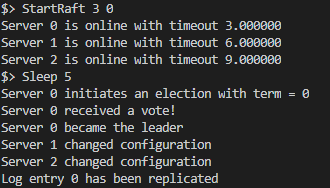
\includegraphics[width=0.4\textwidth,height=45mm]{images/initial_election.png}
\caption{Winning an initial election}
\label{fig:initial_election}
\end{figure}

This test shows that our implementation can hold basic elections in the presence of server failures as long as more than half of the servers present in the configuration are alive. It also shows that elections can time out, leading to another election with an incremented term after another election timeout has elapsed. Finally, it shows that our system can recover from more than half of the servers failing automatically as long as half of them are brought back online eventually.

\texttt{./raft.o < test/test\_election\_dropout.txt} shows election behavior in the presence of a 20\% message drop rate. Dropout messages should be outputted whenever a message is dropped, and some of the initiated elections may time out [Figure \ref{fig:dropout_election}]. Here, the dropout rate is low enough that an election should eventually succeed, and though some of the following heartbeat messages may also be dropped, the system is still able to function normally, albeit with more elections possible.

In the case of network partitioning, if there are an even number of servers, the worst case scenario is an even split of the network (or multiple splits of the network where no one group can form a majority). In this case, no server will ever get elected leader, and the system is still technically safe. For odd server numbers, one partition or the other will always have enough servers to form a majority barring any additional errors. In any case, once the network is restored, the Raft algorithm can successfully elect a leader and continue as usual.

\begin{figure}[htb!]
\centering
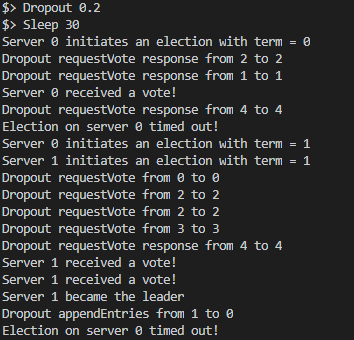
\includegraphics[width=0.4\textwidth,height=75mm]{images/dropout_election.png}
\caption{Simultaneous elections with dropout}
\label{fig:dropout_election}
\end{figure}

%-------------------------------------------------------
\subsection{Log Replication}
%-------------------------------------------------------
\texttt{./raft.o < test/test\_replication.txt} shows how a server that crashed and came back online can catch up its missing log entries from the leader. A cluster of 3 servers is initialized with IDs 0, 1, and 2 and deterministic election timeouts of 3, 6, and 9 seconds respectively. Server 0 becomes the leader after winning the first election, then it quickly crashes before serving any client request. We wait for 7 seconds to ensure server 1 initiates another election and become the new leader. The client sends an update request to server 1 to increase the value of X by 2 using command \texttt{Request 1 X 2}. This request is processed because server 1 is indeed the current leader. After this, server 0 comes back online as a follower. The client further increases the value of X by 3 using command \texttt{Request 1 X 3}. Server 1 crashes after serving this request. However, even though server 1 goes offline, it has replicated its log entries to server 0 and server 2. When server 0 becomes the leader after winning the next election, it will have all log entries server 1 has. We can see this in the last query command \texttt{Request 0 X}. Server 0 correctly replies \texttt{X=5} [Figure \ref{fig:log_replication}].

\begin{figure}[htb!]
\centering
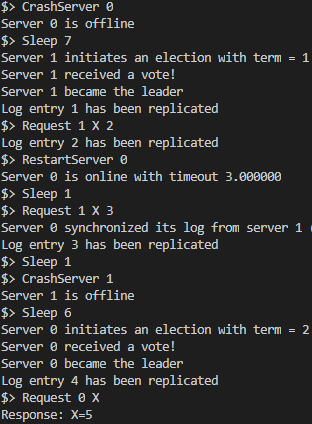
\includegraphics[width=0.40\textwidth,height=90mm]{images/log_replication.png}
\caption{Log replication and persistence after a crash}
\label{fig:log_replication}
\end{figure}

As mentioned earlier in the report, in the presence of message drops, we will retry appending entries enough times that we can be 99.99\% sure that an online server will eventually get the message. Log replication requires a majority of the configuration to respond affirmatively to requests, so network partitions will be a similar case as election, where if at least a majority of servers can respond to RPCs, the system will still be live. If not, safety is still maintained as the leader will not apply changes to the state machine if it is not able to replicate the log. \texttt{test/test\_replication\_dropout} runs a similar test as above but with 10\% message drop probability. The test is non-deterministic, but one should have a high chance of observing the same results most of the time [Figure \ref{fig:log_dropout}].

\begin{figure}[htb!]
\centering
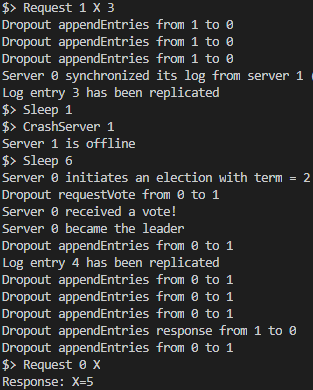
\includegraphics[width=0.40\textwidth,height=90mm]{images/log_dropout.png}
\caption{Log replication in the presence of dropout}
\label{fig:log_dropout}
\end{figure}

%-------------------------------------------------------
\subsection{Membership Change}
%-------------------------------------------------------
\texttt{./raft.o < test/test\_config.txt} [Figure \ref{fig:config_change}] showcases our configuration change procedure. We start with a cluster of 2 servers and write 2 requests to the distributed log, \texttt{X+=10} and \texttt{X-=5}. We then initiate a configuration change to a cluster consisting of server ID's 100, 3, and 2. Regardless if new servers are part of the current cluster or not, the Raft object will handle creation or restarting of the required servers for the membership change. We then see the leader replicating a joint configuration \texttt{0,1-100,3,2} to all servers. Once both server groups respond to the RPC with separate majorities, the leader can write just the new configuration to all servers. Observe that servers 0 and 1 shut down after this log entry is replicated, because they are no longer part of the active configuration. We then crash server 2 and wait for server 3 to be elected. Finally, we query the leader for the value of X and observe that its state machine is correct, even though server 3 was not part of the server group that initially stored these log entries.

Because the membership change process utilizes the existing log replication logic, dropout and network partitioning have the same possible effects as mentioned above. \texttt{test/test\_config\_dropout.txt} shows membership change with overlapping servers, and that it is still achievable at reasonable rates of message dropout.

\begin{figure}[htb!]
\centering
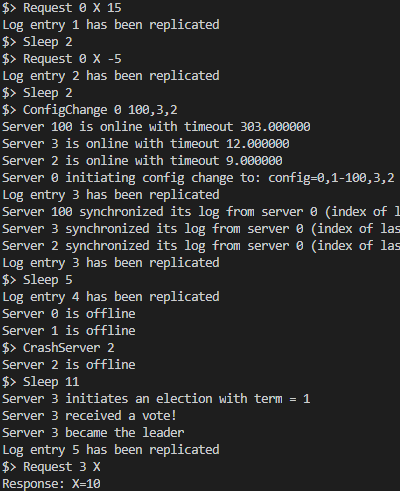
\includegraphics[width=0.45\textwidth,height=115mm]{images/config_change.png}
\caption{Configuration change and log persistence}
\label{fig:config_change}
\end{figure}

%-------------------------------------------------------
\subsection{Note on Randomness}
%-------------------------------------------------------
The tests highlighted in this section set deterministic election timeouts for greater reproducibility, and the tests results including random dropout are naturally non-deterministic. We encourage the reader to run tests from the command line interface with random timeouts (ex. \texttt{StartRaft 4 1}) for more interactivity and interesting scenarios.

%-------------------------------------------------------------------------------
\section{Conclusion}
%-------------------------------------------------------------------------------
We believe we have successfully created a model of a distributed system from scratch and implemented the Raft distributed consensus algorithm on top of it. Our test cases allows us to crash servers between any two client requests. In the real world, server crashes happen in more fine-grained manner. For example, the leader might crash in the middle of handling a client request, and a follower can crash in the middle of replicating its missing log entries from the leader. Our implementation does not allow us to simulate these kinds of server crashes, because we use locks to prevent race conditions for testing purposes. We can reason to our design to argue that some of these crashes should not affect the correctness of our implementation. For example, if a follower crashes in the middle of replicating its missing log entries from the leader, it would simply do the replication again the next time it starts. Without actually deploying our implementation to a real Raft network to try it out, we can not tell for sure that there is not any case in which our implementation works incorrectly, but we believe that these test cases demonstrate a basic working Raft algorithm in action.

\bibliographystyle{plain}
\bibliography{ref}

%%%%%%%%%%%%%%%%%%%%%%%%%%%%%%%%%%%%%%%%%%%%%%%%%%%%%%%%%%%%%%%%%%%%%%%%%%%%%%%%
\end{document}
%%%%%%%%%%%%%%%%%%%%%%%%%%%%%%%%%%%%%%%%%%%%%%%%%%%%%%%%%%%%%%%%%%%%%%%%%%%%%%%%

%%  LocalWords:  endnotes includegraphics fread ptr nobj noindent
%%  LocalWords:  pdflatex acks
